\documentclass{article}
\usepackage{graphicx}
\usepackage{fullpage}
\begin{document}

\title{Fire Dynamics Repository Manual}
\author{M. Currie and B. Quaife}
\maketitle

%\abstract

%This document is meant to make sense of the plots, movies, and scripts located in this repository. The discussions in this document will be organized into four sections: 1) real infrared image data, 2) dynamic mode decomposition (DMD) for the real IR data, 3)  cellular automata (CA) to model the spread of fires, and 4) fire box data, results, etc.

%\pagebreak
\section{Real IR Data}
There are three real data sets that we are working with in the subsequent analyses. 
The datasets are designated 13fsingle1, 13fsingle2, and 13fsingle3, however 
henceforth they shall be referred to as Fire 1, Fire 2, and Fire 3, respectively. Here we 
present basic statistics for each of the three datasets. It is important to note that all 
temperatures are in Celsius.

\begin{table}

\begin{tabular}{|c|c|c|c|c|c|c|}
\hline
 & Mean Temp & Median Temp & Std Dev & Max Temp & Min Temp & Timestep (s) \\
\hline
Fire 1 & 301.939 & 221.310 & 128.379 & 890.108 & 199.998 & 1.000 \\
\hline
Fire 2 & 218.188 & 159.911 & 137.907 & 921.466 & 99.9974 & 1.000 \\
\hline
Fire 3 & 267.044 & 199.998 & 113.061 & 849.827 & 199.998 & 1.000 \\
\hline
\end{tabular}
\centering
\caption{This table shows some basic values for each of the fires. These are overall values, meaning that it looks at all data from all timesteps.}
\end{table}

\subsection{Fire 1}

\begin{figure}
\centering
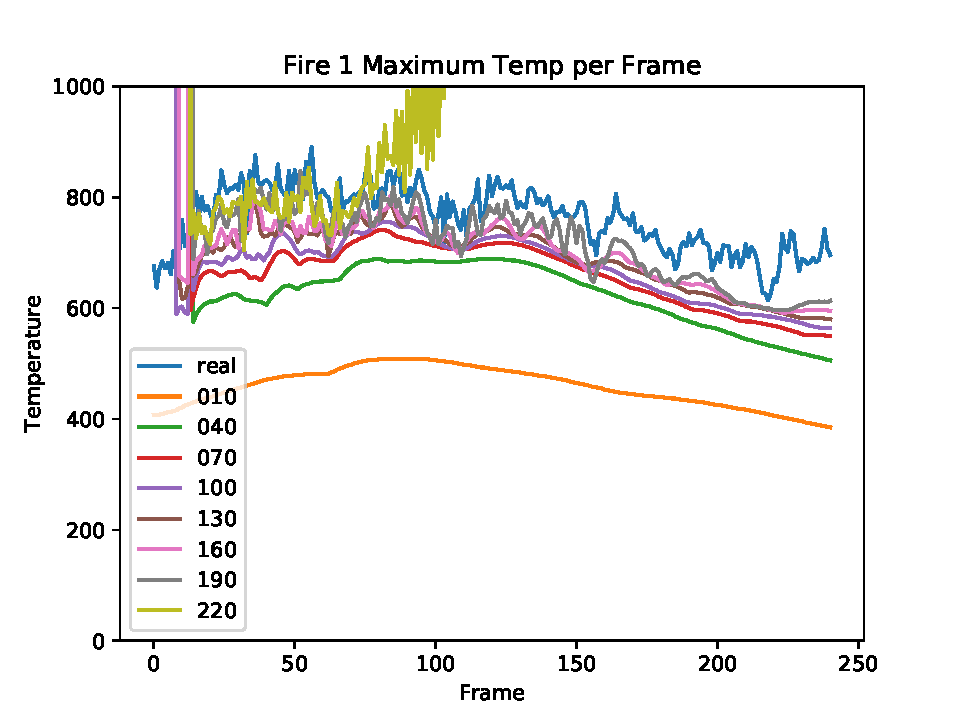
\includegraphics{../plots/f1_maxtemp.pdf}
\caption{hello this is a test}

\end{figure}

\begin{figure}[ht] 
\centering
  \label{ fig7} 
  \begin{minipage}[b]{1\linewidth}
    \centering
    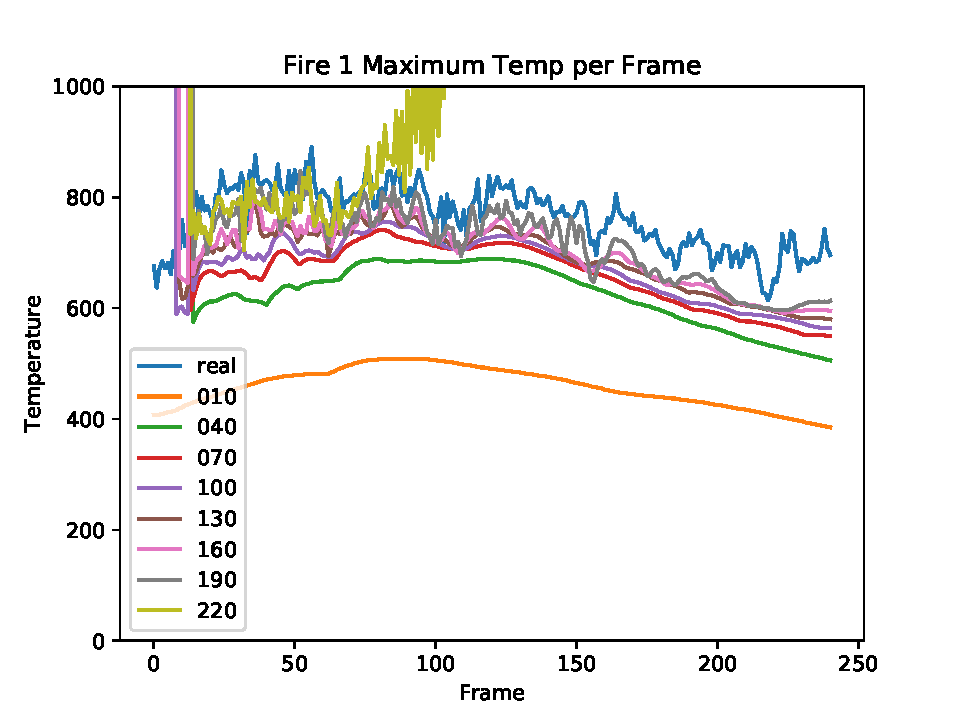
\includegraphics[width=0.8\linewidth]{../plots/f1_maxtemp.pdf} 
    \caption{caption} 
    \vspace{4ex}
  \end{minipage}%%
  \begin{minipage}[b]{1\linewidth}
    \centering
    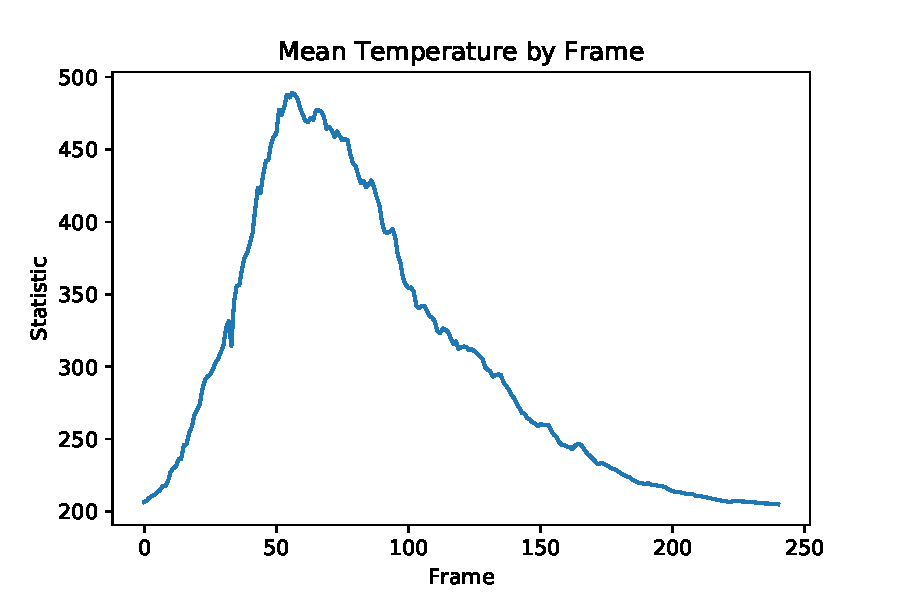
\includegraphics[width=0.8\linewidth]{../plots/f1_meantemp.pdf} 
    \caption{caption} 
    \vspace{4ex}
  \end{minipage} 
  \begin{minipage}[b]{1\linewidth}
    \centering
    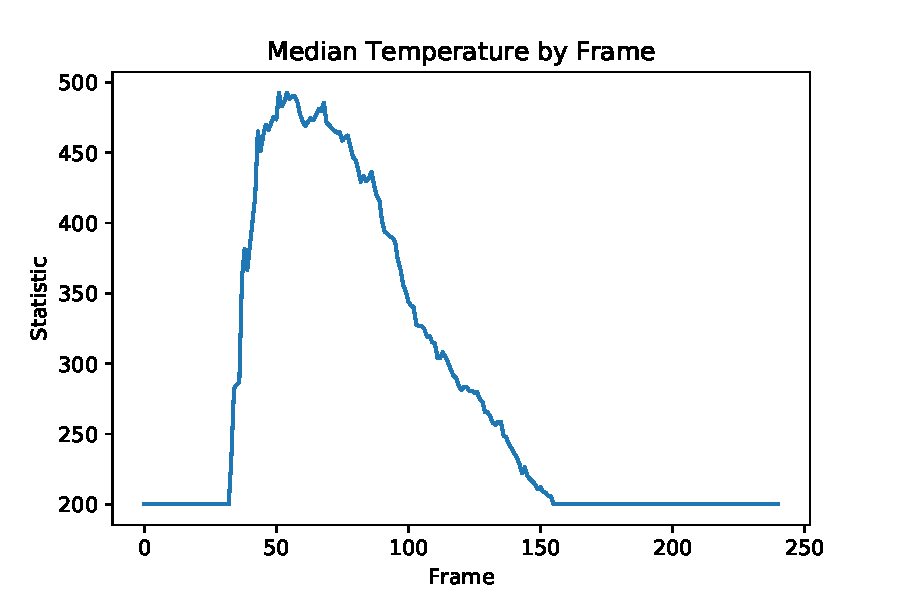
\includegraphics[width=0.8\linewidth]{../plots/f1_mediantemp.pdf} 
    \caption{caption} 
    \vspace{4ex}
  \end{minipage}%% 
  \begin{minipage}[b]{1\linewidth}
    \centering
    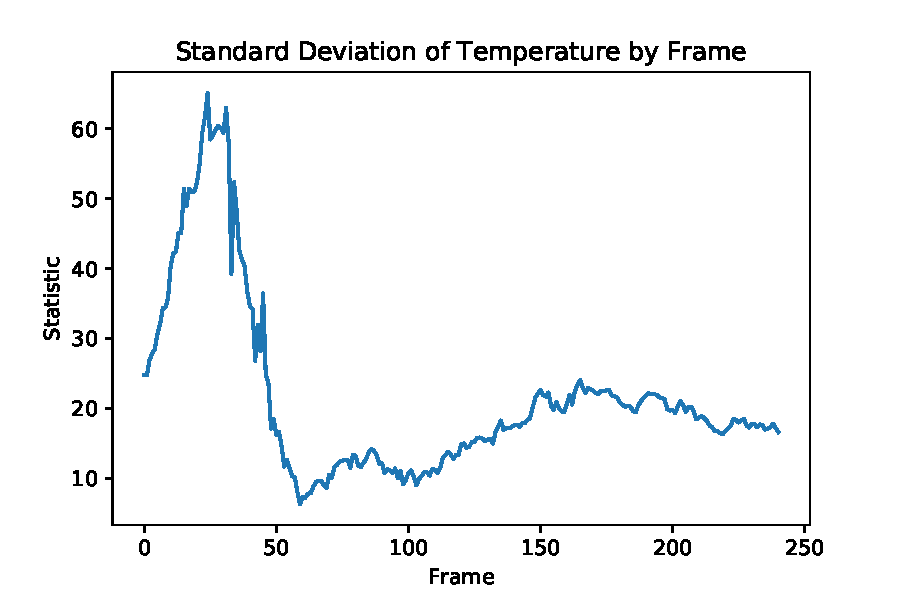
\includegraphics[width=0.8\linewidth]{../plots/f1_stdtemp.pdf} 
    \caption{caption} 
    \vspace{4ex}
  \end{minipage} 
\end{figure}

\subsection{Fire 2}

\subsection{Fire 3}


\end{document}

